\chapter{Software Product Line Configuration \\and Product Generation}
\label{ch:spl configuration}

\section{Software Product Line Configuration}
\label{sec:spl configuration}

The ABS configuration language links feature models, which describe the
structure of a SPL (Chapter~\ref{ch:feature modelling}), to delta modules
(Chapter~\ref{ch:deltas}), which implement behaviour. This link is illustrated
in Fig.~\ref{fig:variability overview}. The configuration defines, for each
selection of features satisfied by the product selection, which delta modules should
be applied to the core. Furthermore, it guides the code generation by ordering
the application of the delta modules.

\begin{figure}
    \centering
    \tikzstyle{box3} = [draw=gray!50, fill=gray!15, thick, rounded corners=1pt]
\tikzstyle{process} = [fill=yellow!90!black, thick, rounded corners=6pt]
\tikzstyle{structure} = [box3, fill=blue!30]
\tikzstyle{behaviour} = [structure, fill=red!40, minimum width=4em]
\tikzstyle{line} =[line width=2\unitlength, black!60, >=latex]
\tikzstyle{thickarrow} =[->,line width=14\unitlength, draw=green!70!black, fill=green!70!black, >=triangle 90 cap]

\begin{tikzpicture}
    [xscale=4.5, yscale=-2.2,
    sm/.style={font=\small,auto}]
    \node[structure] at (1,1) (fm) {Feature Model};
    \node[structure] at (1,3) (ps) {Product Selection};
    \node[process] at (2,2) (conf) {Configuration};
    
    \draw[line,->] (fm) to node[sm] {} (ps);
    \draw[line,dotted,->] (conf) to node[sm,above] {ensures satisfaction} ($(fm)!.5!(ps)$);

    \node[box3,matrix,row sep=2\unitlength,label=above:Modules] at (3,1) (code) {
        \node[behaviour] {Core}; \\ 
        \node[behaviour] {Deltas}; \\
    };

    \node[behaviour] at (3,3) (prod) {Software Product};
    \draw[line] (fm) to (code);
    \draw[line,->,dotted] (conf) to node[sm,sloped,midway,above] {associates} ($(fm)!.5!(code)$);
    \draw[line,dotted,->] (conf) to node[sm] {guides} ($($(code)!.5!(prod)$)!1.5\unitlength!90:(prod)$);

    \draw[thickarrow] (code) to node[sloped,midway,rotate=180,white] {Code Generation} (prod);
\end{tikzpicture}

    \caption{Variability modelling framework of ABS
%   \JP{to Radu: I find hard to explain how a configuration ensures satisfaction. And maybe we should swap FM and PS?}
    }
    \label{fig:variability overview}
\end{figure}

Features and delta modules are associated through \emph{application conditions},
which are logical expressions over the set of features and attributes in a
feature model. The collection of applicable delta modules is given by the
application conditions that are true for a particular feature and attribute
selection. By not associating the delta modules directly with features, a degree
of flexibility is obtained.

\subsection{Syntax}
\label{spl configuration syntax}

The SPL \NT{Configuration} clause specifies the name of the product
line, the set of \NT{Features} it provides, and the set of delta modules used to
implement those features. The feature names are included so that certain simple
self-consistency checks can be performed. The \NT{DeltaClause} is used to
specify each delta module, linking it to the feature model.

\begin{abssyntax}
    \NT{Configuration}
    \concrDefn{ \TR{productline} \NT{TypeId} \TR{;} \NT{Features} \TR{;} \NT{DeltaClauses} }
    \\
    \NT{Features}
    \concrDefn{\TR{features} \fid \MANYG{\TR{,} \fid} }
    \\
    \NT{DeltaClauses}
    \concrDefn{ \MANY{\NT{DeltaClause}} }
    \\
    \NT{DeltaClause}
    \concrDefn{ \TR{delta} \NT{DeltaSpec} \OPT{\NT{AfterCondition}} \OPT{\NT{ApplicationCondition}} \TR{;} }
    \medskip
    \\
    \NT{DeltaSpec}
    \concrDefn{ \NT{TypeName} \OPT{\TR{(} \NT{DeltaParams} \TR{)}} }
    \\
    \NT{DeltaParams}
    \concrDefn{ \NT{DeltaParam} \MANYG{\TR{,} \NT{DeltaParam}} }
    \\
    \NT{DeltaParam}
    \concrDefn{\fid  $|$ \fid.\aid}
%    \concrDefn{\fid  $|$ \fid.\aid  $|$ \NT{DataExp}}
    \\
    \NT{AfterClause}
    \concrDefn{ \TR{after} \NT{TypeName} \MANYG{\TR{,} \NT{TypeName}} }
    \\
    \NT{WhenClause}
    \concrDefn{ \TR{when} \NT{AppCond} }
    \\
    \NT{AppCond}
    \concrDefn{ \NT{AppCond} \TRS{\&\&} \NT{AppCond} }
    \concrCont{ \NT{AppCond} \TRS{||} \NT{AppCond} } 
    \concrCont{ \TR{\sim} \NT{AppCond} } 
    \concrCont{ \TR{(} \NT{AppCond} \TR{)} } 
    \concrCont{ \fid } 
\end{abssyntax}
%
Each delta clause has a \NT{DeltaSpec}, specifying the name of a delta module
name and, optionally, a list of parameters; an \NT{AfterClause}, specifying the
delta modules that the current delta must be applied after; and an application
condition \NT{AppCond}, specifying an arbitrary predicate over the feature and
attribute names in the feature model that describes when the given delta module
is applied.

\subsection{Delta parameters} \label{sec:delta parameters}
A delta clause takes an optional list of \NT{DeltaParams}, which are either
features or fully qualified feature attributes. When a particular
product of the product line is selected (as described in
Section~\ref{sec:product selection}), the value \absinline{true} is assigned to each of
its features and a value is assigned to each of its features' attributes.
These values can be used inside the delta module if the corresponding delta clause
specifies the feature or feature attribute as one of its parameters.


\subsection{Application Conditions}
\label{sec:application conditions}
The configuration is used to specify conditions under which a delta module
should be applied to the core. Such application conditions are propositional
formulas over the set of features and attributes defined by the feature model.
They can be in terms of the presence and absence of features and feature
combinations, as well as attributes of features and integer and boolean
constants. When the propositional formula holds for a given product, the delta
module is applicable. Application conditions are introduced by the \absinline{when}
keyword, as shown in the examples below.
\begin{absexample}
delta D when A or B and ~C;
delta LargeCache when Mem.size > 1024;
\end{absexample}

\subsection{Application Order of Delta Modules}
\label{sec:delta ordering}
For each delta module, the configuration establishes a partial ordering relation
with respect to other deltas by using the \absinline{after} keyword. The partial
order states which delta modules, when applicable, should be applied before the
given delta module.


\subsection{Configuration Example}
A configuration specifies the name of the product line, the set of
features it provides, and the set of delta modules used to implement those
features.

\begin{absexample}
productline MultiLingualHelloWorld;
    features English, German, Dutch, Repeat;
    delta De when German;
    delta Nl when Dutch;
    delta Fr when French;
    delta Rpt(Repeat.times) after De, Nl, Fr when Repeat;
\end{absexample}

The example above first names the set of features from the feature model (cf.
Section~\ref{sec:feature model example}) used to configure this product line.
The \absinline{delta} clauses link each delta module to the feature model
through an application condition (\absinline{when} clause); in this case, a
delta module is applied simply when the specified feature is selected (e.g.
``\absinline{De when German}''). There is no delta module corresponding to the
feature \absinline{English}, as the core module provides support for the English
language by default. In addition, \absinline{Rpt} has to be applied
\absinline{after} \absinline{De}, \absinline{Nl} and \absinline{Fr}.
The \absinline{Rpt} delta has a parameter \absinline{Repeat.times}, the
\absinline{times} attribute of the feature \absinline{Repeat}; its value
(defined by product selection, see Section~\ref{sec:product selection}) is
propagated to the \absinline{Rpt} delta as described in Section~\ref{sec:delta parameters}.


\section{Product Generation}
\label{sec:product generation}

The process of generating a software product from a given software product line
relies on the full ABS specification of an SPL, that is, a feature model with a
set of product declarations (Chapter~\ref{ch:feature modelling}), a set of delta
modules (Chapter~\ref{ch:deltas}), and a configuration that connects the two
(Section~\ref{sec:spl configuration} above).
To generate a particular product, this has to be selected either using the
Eclipse IDE (cf. Figure~\ref{fig:eclipse product generation}), or given as an argument when invoking the compiler
on the command line. For example:

\begin{cmdline}
generateJava -product=P2 Hello.abs
\end{cmdline}

\begin{figure}[htp]
	\centering
	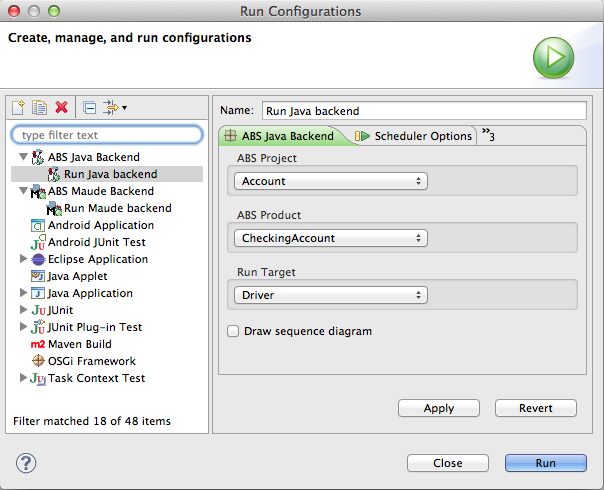
\includegraphics[width=.9\linewidth]{fig/eclipse-product-generation}
	\caption{SPL product generation using the Eclipse IDE}
 	\label{fig:eclipse product generation}
\end{figure}

\subsection{Example}

For example, selecting the product \absinline{P2} of the ``Hello world'' product line
triggers the compiler to execute through the following steps.

\begin{enumerate}
    \item Check if the product is valid with respect to the feature model. 
    In this case the product \absinline{P2} is valid.

    \item Find all applicable delta modules. In this case the deltas modules
    with an application condition that holds are \absinline{Nl} and
    \absinline{Rpt(3)}.
  
    \item Linearise the application order of delta modules. The restriction here
    is over the delta module \absinline{Rpt}, which has to follow any of the
    language deltas.
  
    \item Apply the deltas sequentially. First, the \absinline{Nl} delta is applied
    to the Core ABS program. Then the \absinline{Rpt(3)} delta is applied to
    the result of the previous application.
\end{enumerate}

\noindent The result is a core ABS program.
